\documentclass[a4paper,12pt, fleqn]{article}
\usepackage{amsmath}
\usepackage[hmargin=1in,vmargin=1in]{geometry}
\usepackage{enumerate}
\usepackage{graphicx,float}
\usepackage{hyperref}
\usepackage{listings}
\pagestyle{empty}
\linespread{1.5}
\begin{document}
\begin{center}
\Large
\textbf{AMATH 481/581 - Autumn 2022}
\textbf{Homework \#4}
\textbf{Sathvik Chinta}
\normalsize
\end{center}
\begin{enumerate}
    \item 
        \textbf{Presentation Skills:} 2D plotting \\
        \begin{figure}[H]
            \centering
            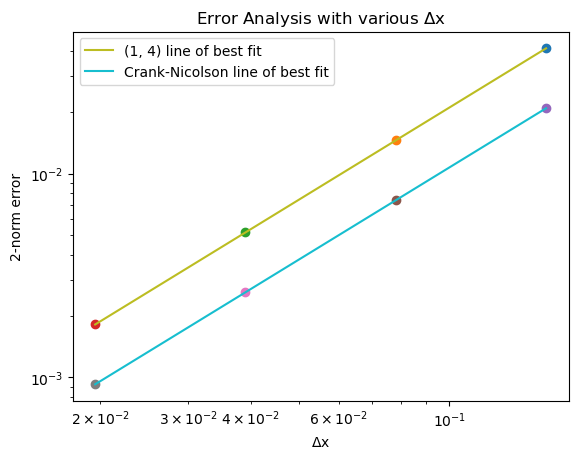
\includegraphics[width=0.45\textwidth]{/workspaces/AMATH-481/Homework/error_analysis.png}
            \caption{log-log plot of different $\Delta$x values against the two norm error for the (1, 4) accurate method
            against the (2, 2) accurate method (Crank-Nicolson). At every $\Delta$x value, the two norm error 
            for the Crank-Nicolson is lower than the two norm error for the (1, 4) accurate method. This shows that
            the trade off between the temporal (1st order accurate vs 2nd order accurate) and spatial (2nd order accurate vs 4th order accurate)
            is a fine balance as they both have almost the same slope in the log-log plot (~1.5).}
            \label{fig:hw4-1a}
        \end{figure}
        
        \textbf{Appendix: Code}: \\
        \begin{lstlisting}[basicstyle=\tiny]
        [language=Python]
            import numpy as np
            import scipy.sparse
            import scipy.optimize
            import matplotlib.pyplot as plt
            alpha = 2
            L = 10
            Time = 2
            n = 128
            xspan, dx = np.linspace(-L, L, n, endpoint=False, retstep=True)
            tspan, dt = np.linspace(0, Time, 501, retstep=True)
            lambda_star = (alpha * dt) / (dx**2)
            # %%
            e1 = -30 * np.ones(n)
            e2 = 16 * np.ones(n)
            e3 = -1 * np.ones(n)
            A = scipy.sparse.spdiags([e3, e2, e1, e2, e3],
                                    [-2, -1, 0, 1, 2], n, n, format='csc')
            A[0, -1] = 16
            A[0, -2] = -1
            A[1, -1] = -1
            A[-1, 0] = 16
            A[-1, 1] = -1
            A[-2, 0] = -1

            A = 1/12 * A
            A3 = A.toarray()

            # Solve
            sol1 = np.zeros((len(xspan), len(tspan)))
            u0 = 10 * np.cos(2 * np.pi * xspan / L) + 30 * np.cos(8 * np.pi * xspan / L)
            sol1[:, 0] = u0
            for i in range(len(tspan) - 1):
                u1 = u0 + lambda_star * (A@u0)
                sol1[:, i + 1] = u1 
                u0 = u1
            A5 = sol1[:, -1]
            #reshape A5 to a 128x1 matrix
            A5 = A5.reshape(128,1)

            # %%
            # Question 2
            e1 = -2 * np.ones(n)
            e2 = np.ones(n)
            mid = 1/2 * lambda_star * scipy.sparse.spdiags([e2, e1, e2],
                                                        [-1, 0, 1], n, n, format='csc')

            mid[0, -1] = 1/2 * lambda_star
            mid[-1, 0] = 1/2 * lambda_star
            B = scipy.sparse.eye(n) - mid
            C = scipy.sparse.eye(n) + mid
            A7 = B.toarray()
            A8 = C.toarray()
            print(A8)
            # %%
            # Solve suing LU decomposition 
            sol2 = np.zeros((len(xspan), len(tspan)))
            u0 = 10 * np.cos(2 * np.pi * xspan / L) + 30 * np.cos(8 * np.pi * xspan / L)
            sol2[:, 0] = u0
            PLU = scipy.sparse.linalg.splu(B)
            test = PLU.solve(C@u0)
            for i in range(len(tspan) - 1):
                u1 = PLU.solve(C@u0)
                sol2[:, i + 1] = u1
                u0 = u1
            A9 = sol2[:, -1]
            # reshape A9 to a 128x1 matrix
            A9 = A9.reshape(128,1)
            print(A9)

            A10 = 0 

            # %%
            # Question 3
            #Load the exact solution from the file exact_128.csv 
            exact = np.loadtxt('exact_128.csv', delimiter=',')
            #reshape the exact solution to a 128x1 matrix
            exact = exact.reshape(128,1)
            #find the two norm difference between A5 and exact, save as A11
            A11 = np.linalg.norm(A5 - exact)
            #find the two norm difference between A9 and exact, save as A12
            A12 = np.linalg.norm(A9 - exact)

            # %%
            # redo both problems with n = 256, load in the exact solution from the file exact_256.csv
            n = 256
            xspan, dx2 = np.linspace(-L, L, n, endpoint=False, retstep=True)
            tspan, dt = np.linspace(0, Time, (4 * 500) + 1, retstep=True)
            e1 = -30 * np.ones(n)
            e2 = 16 * np.ones(n)
            e3 = -1 * np.ones(n)
            A = scipy.sparse.spdiags([e3, e2, e1, e2, e3],
                                    [-2, -1, 0, 1, 2], n, n, format='csc')

            A[0, -1] = 16
            A[0, -2] = -1
            A[1, -1] = -1
            A[-1, 0] = 16
            A[-1, 1] = -1
            A[-2, 0] = -1

            A = 1/12 * A
            print(A.toarray())
            sol1 = np.zeros((len(xspan), len(tspan)))
            u0 = 10 * np.cos(2 * np.pi * xspan / L) + 30 * np.cos(8 * np.pi * xspan / L)
            sol1[:, 0] = u0
            for i in range(len(tspan) - 1):
                u1 = u0 + lambda_star * (A@u0)
                sol1[:, i + 1] = u1 
                u0 = u1
            first = sol1[:, -1]
            # %%
            e1 = -2 * np.ones(n)
            e2 = np.ones(n)
            mid = 1/2 * lambda_star * scipy.sparse.spdiags([e2, e1, e2],
                                                            [-1, 0, 1], n, n, format='csc')
            #mid = scipy.sparse.lil_matrix(mid)
            mid[0, -1] = 1/2 * lambda_star
            mid[-1, 0] = 1/2 * lambda_star
            B = scipy.sparse.eye(n) - mid
            C = scipy.sparse.eye(n) + mid
            # Solve suing LU decomposition
            sol2 = np.zeros((len(xspan), len(tspan)))
            u0 = 10 * np.cos(2 * np.pi * xspan / L) + 30 * np.cos(8 * np.pi * xspan / L)
            sol2[:, 0] = u0
            PLU = scipy.sparse.linalg.splu(B)
            for i in range(len(tspan) - 1):
                u1 = PLU.solve(C@u0)
                sol2[:, i + 1] = u1
                u0 = u1
            second = sol2[:, -1]
            #Load the exact solution from the file exact_256.csv
            exact = np.loadtxt('exact_256.csv', delimiter=',')
            #find the two norm difference between A5 and exact, save as A11
            A13 = np.linalg.norm(first - exact)
            #find the two norm difference between second and exact, save as A12
            A14 = np.linalg.norm(second - exact)

            # %%
            # redo both problems with n = 512, load in the exact solution from the file exact_512.csv
            n = 512
            xspan, dx3 = np.linspace(-L, L, n, endpoint=False, retstep=True)
            tspan, dt = np.linspace(0, Time, (16 * 500) + 1, retstep=True)
            e1 = -30 * np.ones(n)
            e2 = 16 * np.ones(n)
            e3 = -1 * np.ones(n)
            A = scipy.sparse.spdiags([e3, e2, e1, e2, e3],
                                        [-2, -1, 0, 1, 2], n, n, format='csc')

            A[0, -1] = 16
            A[0, -2] = -1
            A[1, -1] = -1
            A[-1, 0] = 16
            A[-1, 1] = -1
            A[-2, 0] = -1

            A = 1/12 * A
            print(A.toarray())
            sol1 = np.zeros((len(xspan), len(tspan)))
            u0 = 10 * np.cos(2 * np.pi * xspan / L) + 30 * np.cos(8 * np.pi * xspan / L)
            sol1[:, 0] = u0
            for i in range(len(tspan) - 1):
                u1 = u0 + lambda_star * (A@u0)
                sol1[:, i + 1] = u1 
                u0 = u1
            first = sol1[:, -1]
            # %%
            e1 = -2 * np.ones(n)
            e2 = np.ones(n)
            mid = 1/2 * lambda_star * scipy.sparse.spdiags([e2, e1, e2],
                                                            [-1, 0, 1], n, n, format='csc')
            #mid = scipy.sparse.lil_matrix(mid)
            mid[0, -1] = 1/2 * lambda_star
            mid[-1, 0] = 1/2 * lambda_star
            B = scipy.sparse.eye(n) - mid
            C = scipy.sparse.eye(n) + mid
            # Solve suing LU decomposition
            sol2 = np.zeros((len(xspan), len(tspan)))
            u0 = 10 * np.cos(2 * np.pi * xspan / L) + 30 * np.cos(8 * np.pi * xspan / L)
            sol2[:, 0] = u0
            PLU = scipy.sparse.linalg.splu(B)
            for i in range(len(tspan) - 1):
                u1 = PLU.solve(C@u0)
                sol2[:, i + 1] = u1
                u0 = u1
            second = sol2[:, -1]
            #Load the exact solution from the file exact_512.csv
            exact = np.loadtxt('exact_512.csv', delimiter=',')
            #find the two norm difference between A5 and exact, save as A11
            A15 = np.linalg.norm(first - exact)
            #find the two norm difference between second and exact, save as A12
            A16 = np.linalg.norm(second - exact)

            # %%
            # redo both problems with n = 1024, load in the exact solution from the file exact_1024.csv
            n = 1024
            xspan, dx4 = np.linspace(-L, L, n, endpoint=False, retstep=True)
            tspan, dt = np.linspace(0, Time, (64 * 500) + 1, retstep=True)
            e1 = -30 * np.ones(n)
            e2 = 16 * np.ones(n)
            e3 = -1 * np.ones(n)
            A = scipy.sparse.spdiags([e3, e2, e1, e2, e3],
                                        [-2, -1, 0, 1, 2], n, n, format='csc')

            A[0, -1] = 16
            A[0, -2] = -1
            A[1, -1] = -1
            A[-1, 0] = 16
            A[-1, 1] = -1
            A[-2, 0] = -1

            A = 1/12 * A
            print(A.toarray())
            sol1 = np.zeros((len(xspan), len(tspan)))
            u0 = 10 * np.cos(2 * np.pi * xspan / L) + 30 * np.cos(8 * np.pi * xspan / L)
            sol1[:, 0] = u0
            for i in range(len(tspan) - 1):
                u1 = u0 + lambda_star * (A@u0)
                sol1[:, i + 1] = u1 
                u0 = u1
            first = sol1[:, -1]
            # %%
            e1 = -2 * np.ones(n)
            e2 = np.ones(n)
            mid = 1/2 * lambda_star * scipy.sparse.spdiags([e2, e1, e2],
                                                            [-1, 0, 1], n, n, format='csc')
            #mid = scipy.sparse.lil_matrix(mid)
            mid[0, -1] = 1/2 * lambda_star
            mid[-1, 0] = 1/2 * lambda_star
            B = scipy.sparse.eye(n) - mid
            C = scipy.sparse.eye(n) + mid
            # Solve suing LU decomposition
            sol2 = np.zeros((len(xspan), len(tspan)))
            u0 = 10 * np.cos(2 * np.pi * xspan / L) + 30 * np.cos(8 * np.pi * xspan / L)
            sol2[:, 0] = u0
            PLU = scipy.sparse.linalg.splu(B)
            for i in range(len(tspan) - 1):
                u1 = PLU.solve(C@u0)
                sol2[:, i + 1] = u1
                u0 = u1
            second = sol2[:, -1]
            #Load the exact solution from the file exact_1024.csv
            exact = np.loadtxt('exact_1024.csv', delimiter=',')
            #find the two norm difference between A5 and exact, save as A11
            A17 = np.linalg.norm(first - exact)
            #find the two norm difference between second and exact, save as A12
            A18 = np.linalg.norm(second - exact)

            # %%
            #plot the norms of dx, dx2, dx3, and dx4 against A11, A13, A15, A17 on a loglog plot

            fig, ax = plt.subplots()
            ax.loglog(dx, A11, 'o')
            ax.loglog(dx2, A13, 'o')
            ax.loglog(dx3, A15, 'o')
            ax.loglog(dx4, A17, 'o')
            ax.loglog(dx, A12, 'o')
            ax.loglog(dx2, A14, 'o')
            ax.loglog(dx3, A16, 'o')
            ax.loglog(dx4, A18, 'o')
            ax.set_xlabel('$\Delta$x')
            ax.set_ylabel('2-norm error')
            #set the title of the plot to be '(1, 4) method error analysis with various dx'
            ax.set_title('Error Analysis with various $\Delta$x')
            #make a line of best fit for the data
            m, b = np.polyfit(np.log([dx, dx2, dx3, dx4]), np.log([A11, A13, A15, A17]), 1)
            ax.loglog([dx, dx2, dx3, dx4], np.exp(m * np.log([dx, dx2, dx3, dx4]) + b), label='(1, 4) line of best fit')
            m, b = np.polyfit(np.log([dx, dx2, dx3, dx4]), np.log([A12, A14, A16, A18]), 1)
            ax.loglog([dx, dx2, dx3, dx4], np.exp(m * np.log([dx, dx2, dx3, dx4]) + b), label='Crank-Nicolson line of best fit')
            ax.legend()
            plt.show()

            plt.savefig('error_analysis.png')

        \end{lstlisting}

    \item 
        \textbf{Presentation Skills:} 3D plotting \\
        \begin{figure}[H]
            \centering
            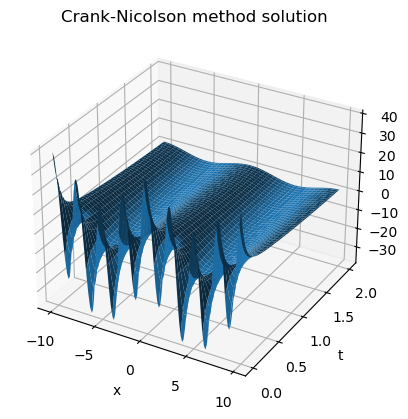
\includegraphics[width=0.45\textwidth]{/workspaces/AMATH-481/Homework/Crank-Nicolson method solution.png}
            \caption{3d plot of the entire final solution with n = 128 for the most accurate method (Crank-Nicolson). 
            The plot shows that near t = 0, the solution is much more chaotic and fluctuates wildly. In contrast, as time
            progresses, the solution becomes much more smooth and the heat becomes more normalized. This signifies the heat is spreading out and becoming more uniform through the rod.}
            \label{fig:hw4-1b}
        \end{figure}

        \textbf{Appendix: Code}: \\
        \begin{lstlisting}[basicstyle=\tiny]
        [language=Python]
            # %%
            import numpy as np
            import scipy.sparse
            import scipy.optimize
            import matplotlib.pyplot as plt
            # %%
            # Question 1
            alpha = 2
            L = 10
            Time = 2
            n = 128
            xspan, dx = np.linspace(-L, L, n, endpoint=False, retstep=True)
            tspan, dt = np.linspace(0, Time, 501, retstep=True)
            lambda_star = (alpha * dt) / (dx**2)
            # %%
            e1 = -30 * np.ones(n)
            e2 = 16 * np.ones(n)
            e3 = -1 * np.ones(n)
            A = scipy.sparse.spdiags([e3, e2, e1, e2, e3],
                                    [-2, -1, 0, 1, 2], n, n, format='csc')
            A[0, -1] = 16
            A[0, -2] = -1
            A[1, -1] = -1
            A[-1, 0] = 16
            A[-1, 1] = -1
            A[-2, 0] = -1
            
            A = 1/12 * A
            A3 = A.toarray()
            
            # Solve
            sol1 = np.zeros((len(xspan), len(tspan)))
            u0 = 10 * np.cos(2 * np.pi * xspan / L) + 30 * np.cos(8 * np.pi * xspan / L)
            sol1[:, 0] = u0
            for i in range(len(tspan) - 1):
                u1 = u0 + lambda_star * (A@u0)
                sol1[:, i + 1] = u1 
                u0 = u1
            A5 = sol1[:, -1]
            #reshape A5 to a 128x1 matrix
            A5 = A5.reshape(128,1)
            # %%
            # stability analysis
            g = lambda z: 1 + 1/12 * lambda_star * (-30 + 32 * np.cos(z) - 2 * np.cos(2 * z))
            A1 = abs(g(1))
            minimum_index = scipy.optimize.fminbound(lambda z: -abs(g(z)), -np.pi, np.pi)
            A2 = g(minimum_index)
            
            # %%
            # Question 2
            e1 = -2 * np.ones(n)
            e2 = np.ones(n)
            mid = 1/2 * lambda_star * scipy.sparse.spdiags([e2, e1, e2],
                                                        [-1, 0, 1], n, n, format='csc')
            
            mid[0, -1] = 1/2 * lambda_star
            mid[-1, 0] = 1/2 * lambda_star
            B = scipy.sparse.eye(n) - mid
            C = scipy.sparse.eye(n) + mid
            A7 = B.toarray()
            A8 = C.toarray()
            print(A8)
            # %%
            # Solve suing LU decomposition 
            sol2 = np.zeros((len(xspan), len(tspan)))
            u0 = 10 * np.cos(2 * np.pi * xspan / L) + 30 * np.cos(8 * np.pi * xspan / L)
            sol2[:, 0] = u0
            PLU = scipy.sparse.linalg.splu(B)
            test = PLU.solve(C@u0)
            for i in range(len(tspan) - 1):
                u1 = PLU.solve(C@u0)
                sol2[:, i + 1] = u1
                u0 = u1
            A9 = sol2[:, -1]
            # reshape A9 to a 128x1 matrix
            A9 = A9.reshape(128,1)
            print(A9)
            
            A10 = 0 
            # %%
            # make a 3d plot of the solution of sol2 
            fig = plt.figure()
            ax = fig.add_subplot(111, projection='3d')
            X, T = np.meshgrid(xspan, tspan)
            ax.plot_surface(X, T, sol2.T)
            ax.set_xlabel('x')
            ax.set_ylabel('t')
            ax.set_zlabel('u')
            ax.set_title('Crank-Nicolson method solution')
            plt.show()

        \end{lstlisting}

\end{enumerate}
    
\end{document}